% vim: tw=80

\chapter{Theoretical Foundations}
\label{sec:theoretical_foundations}

A deeper understanding about physical principles relies always on the interplay
of the theoretical predictions and accompanying experimental meausurements.
Theoretical models try to describe the behaviour of nature and have to be
confirmed or excluded in precise measurements.

This chapter shortly summarizes the Standard Model of particle physics, with a
focus on quantum chromodynamics (QCD), the theory describing the strong
interaction.

\section{Standard Model of Particle Physics}

The Standard Model of particle physics (SM) is a comprehensive theoretical
concept which describes the fundamental particles and their interactions from
basic principles. The SM is founded on the concept of quantum field theories, in
which the interaction between particles are mediated by quantized gauge fields.

Each of the fundamental spin-$\sfrac{1}{2}$ particles, also known as fermions,
has a corresponding antiparticle with same properties but opposite sign of
quantum bumbers. They are classified in three families and carry quantum numbers
of electric charge $Q$, weak isospin $T$ and color. The weak hypercharge $Y_W$
is related to the weak isospin and the electric charge by $Y_W = 2(Q-T_3)$. The
quantum numbers define the coupling of the fermions. There are four fundamental
forces of which three are considered in the SM.

The electromagnetic and weak force are described by a $U(1)\times SU(2)$
symmetry, which is spontaneously broken by the coupling to the scalar Higgs
field. The gauge bosons of the unified electroweak theory are a mixture
resulting in massize $W^\pm$ and the $Z^0$ boson and the massless photon. The
eigenstates of the weak interaction differ from the mass eigenstates and can be
calculated by rotating the mass-eigenstates using the CKM
matrix~\cite{Cabibbo:1963yz,Kobayashi:1973fv}. The
same effect is observed in the lepton sector in which the mass eigenstates of
the neutrinos do not match the interaction eigenstates leading to oscillations
between neutrino flavors. The analogue matrix is called PMNS
matrix~\cite{Maki:1962mu,Pontecorvo:1957qd}.

The strong force is described by the unbroken $\mathrm{SU}(3)$ color gauge
theory, called quantum chromodynamics. There are eight gauge bosons, the gluons,
which carry color charge. 

The Higgs boson, the field quanta of the Higgs field which causes the
electroweak symmetry breaking and  was predicted for a long time by theorists.
Recently, it was discovered in at the LHC~\cite{Chatrchyan:2012xdj,Aad:2012tfa}.



% \todo{check t3 of gluon, compare with joram thesis}
% \begin{table}[htb]
% \centering
% \caption[The gauge bosons and their properties]{The properties of the gauge
% bosons mediating the four fundamental interaction forces in the Standard Model:
% The mass, the spin and parity, the charge and the weak isospin.}
% \label{tab:fundamental_interactions}
% \begin{tabular}{lcccccc} \toprule
% Interaction                         & Range (m)                   & Vector boson & Mass (\si{\giga \electronvolt})   & $J^P$ & Q (e)  & $T_3$\\\midrule
% electromanetism                     & $\infty$                    & $\gamma$     & 0                                 & $1^-$ & 0      & 0\\
% \multirow{2}{*}{weak interaction}   & \multirow{2}{*}{$10^{-13}$} & $Z$          & 91.19                             & 1     & 0      & 0\\
%                                     &                             & $W^\pm$      & 80.40                             & 1     & $\pm$e & $\pm$1\\
% strong                              & $10^{-15}$                  & gluons       & 0                                 & $1^-$ & 0      & 0\\\bottomrule
% \end{tabular}
% \end{table}

\section{Quantum Chromodynamics}

Quantum chromodynamics (QCD) is the theory of the strong interaction. It
describes the interaction between quarks and gluons, the fundamental particles
which make up hadrons.

\begin{equation*}
    F_{\mu\nu}^A = \partial_\mu 
\end{equation*}<++>


\begin{figure}[htb] 
    \centering
    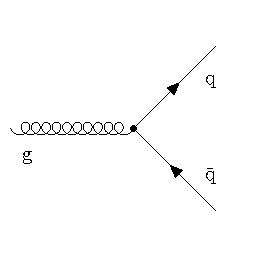
\includegraphics[width=0.33\textwidth]{figures/drawings/feynman/gqq.pdf}\hfill
    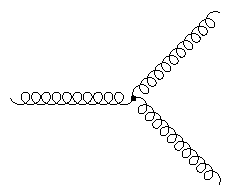
\includegraphics[width=0.33\textwidth]{figures/drawings/feynman/ggg.pdf}\hfill
    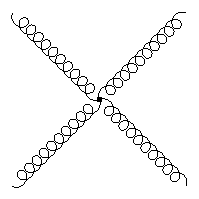
\includegraphics[width=0.33\textwidth]{figures/drawings/feynman/gggg.pdf}\hfill
    \caption[Fundamental vertices of QCD]{The fundamental Feynman rules of QCD
    comprise a quark-antiquark-gluon vertex, a three-gluon vertex and a 4-gluon
    vertex. The first two are proportional to $g_\mathrm{S}$, the last one
    proportional to $g_\mathrm{S}^2$.} 
    \label{fig:fundamental_couplings} 
\end{figure}



\section{Renormalization}

\begin{equation} 
    \mur^2 \frac{d}{d \mur^2} X \left(\frac{Q^2}{\mur^2},\as(\mur^2)\right) = \left(
    \mur^2 \frac{\partial X}{\partial \mur^2} + \mur^2 \frac{\partial
    \as(\mu^2)}{\partial \mur^2} \frac{\partial X}{\partial \as(\mu^2)} \right) \stackrel{!}{=} 0 
\end{equation}


\begin{equation}
    \mur^2 \frac{d \as}{d \mur^2} = \beta(\as) = - \left( \beta_0 \as^2 + \beta_1 \as^3
    + \beta_2 \as^4 + \ldots \right)
\end{equation}

\begin{equation} 
    \beta_0 = \frac{33 - 2 n_f}{12\pi}
\end{equation}

\begin{equation} 
    \beta_1 = \frac{153 - 19 n_f}{24\pi^2}
\end{equation}

\begin{equation} 
   \beta_2 = \frac{2857 -\left(\sfrac{5033}{9}\right)n_f + \left(\sfrac{335}{27}
   \right)n_f^2}{128 \pi^3}
\end{equation}

\begin{equation*}
   \as(\mur^2) = \frac{1}{\beta_0 \ln \left( \sfrac{\mur^2}{\Lambda^2} \right)}
\end{equation*}


alphas from mz

\begin{equation*}
   \as\left(\mur, \as(\mz)\right) = \frac{\as(\mz)}{1 + \as(\mz)\beta_0 \ln
       \left( \sfrac{\mur^2}{\mz^2} \right)}
\end{equation*}


\todo{scale dependence of perturbative series}
\todo{scale dependence of the cross section}

\section{Running of the Strong Coupling}

\begin{equation*}
    \frac{\partial f_a (x, \muf^2)}{\partial \muf^2} = \sum_b \frac{\as(\muf^2)}{2 \pi} \int_x^1
    \frac{d \zeta}{\zeta} P_{ab} \left(\frac{x}{\zeta},
    \as(\muf^2)\right) f_b(\zeta, \muf)
\end{equation*}



\section{Factorization and Parton Density Functions}

The perturbative series is only converging for $\as(\mur) \ll 1$. As this is not
given for low energies, perturbative calculations are not applicable in this
energy regime. 

The \emph{factorization theorem} separates the short-distance interactions,
which are calculated in the hard matrix element, from long-distance
interactions at an additionally introduced factorization scale \muf. This soft
part of the interaction is defined by the parton distributions in the proton.

The cross section calculation 

\subsection{Factorization theorem}


\subsection{DGLAP Evolution Equations}


\subsection{Parton Distribution Functions}

The structure of the proton is described by parton distribution functions
(PDFs).
They represent the probability density\footnote{more precise a number density as
the pDFs are normalized to the number of partons} to find a parton carrying a momentum
fraction $x$ of the proton momentum at a squared energy scale $Q^2$. 

The DGLAP equations describe the evolution of the PDFs from a starting scale
$Q_0$ to an arbitray scale $Q$. However, the $x$-dependence of the PDFs as well
as the PDFs themselves at the starting scale $Q_0$ cannot be calculated, but
have to be derived from fits to data from experiments.

Several groups determine the proton PDFs in global fits to a large variety of
measurements from different experiments. Instead of determining all the 13 quark,
antiquark and gluon PDFs independently, the number can be reduced by choosing a
sufficiently low starting scale $Q_0$ below the threshold of the charm quark
mass and calculating the heavy flavour PDFs in a heavy flavour
scheme~\cite{rt_scheme}. Furthermore the PDF of the top and anti-top quark is
often neglected due to its large rest-mass. In the fits, each parton is
parametrized with sufficiently flexible function to the describe the $x$
dependence at the starting scale $Q_0$. The PDFs are evolved to the higher
scales of each measurement and the PDF parameters are adapted in an iterative
$\chisq$ fit.

Global PDFs are determined by the
CTEQ~\cite{Dulat:2015mca},MMHT~\cite{Harland-Lang:2014zoa},
NNPDF~\cite{Ball:2014uwa} and the ABM~\cite{Alekhin:2013nda} groups at LO, NLO
and NNLO. While the measurements which are put into the fit are often similar,
there are differences in the applied minimization method, phenomenological
approaches and the estimation of the uncertainties. More details are given in
Sec.~\ref{sec:pdf_uncertainties} in which the uncertainy of the PDFs on the
cross section measurement is discussed.

The HERAPDF group~\cite{Abramowicz:2015mha} uses a slightly different approach
by using a less flexible parameterization but restricting the data to
measurements from the HERA experiments, which provide a very precise and
compatible dataset. Furthermore the HERAPDF group released their fitting
framework HERAFitter~\cite{Alekhin:2014irh} as open source software, which can
be used by anyone.  HERAFitter is employed in Sec.~\ref{sec:pdf_constraints} to
study the constraints of the triple differential dijet measurements on the PDFs.

\section{Hadronization and Parton Shower}

As perturbative QCD calculations lack the capabilities of describing the
soft component of the interaction, additional models are employed which describe
the emission of additional partons and the hadronization into color-less bound
states. 

\subsection{Parton showers}

The accelerated colored partons undergo subsequent emission of gluons. Unlike in
QED radiation, gluons themselves carry color charge and therefore also emit
further gluons, leading to the parton shower. 

The dominant contributions come from collinear parton splitting and soft gluon
emissions. The collinear splitting of a parton is described by splitting
functions which are identical to the DGLAP splitting functions. The
subsequential application of the splitting to the colored particles leads to the
parton shower. The evolution of the shower is determined by an evolution
variable, \eg the virtual-mass squared of the partons in the shower. The upper
limit on the initial virtuality is given by the momentum transfer scale of the
hard process while the shower is terminated when the virtualities fall below the
hadronization scale, which is of the order of $\SI{1}{\GeV}$.

Actually the parton shower mimics the effect of effect of higher-order
corrections. As they are often not feasible to be calculated, the parton shower
approximation is instead used. Though great take has to be taken to avoid any
double counting if using a NLO generator in combination with a parton shower.


\subsection{Hadronization}

The result of the parton shower is a large number of color charged particles. As
color charged particles cannot be observed, they have to hadronize into bound
states which are color-less. The MC event generators Pythia and Herwig employ
different models to simulate the hadronization process. Pythia uses the Lund
string fragmentation model while Herwig is based on the cluster fragmentation
model.

\paragraph{Lund String Fragmentation Model}

Within the Lund string model, the attraction between a $q\bar q$ pair is
modeled through string, whose energy follows a coulomb potential as a function
of the distance between the two quarks. Final-state gluons from the parton
shower are considered as kinks in the strings. If the string exceeds a certain
threshold, it breaks up and new quark-antiquark pairs are formed. If the
available energy is too small, the quarks and antiquarks recombine into mesons
and baryons.

\paragraph{Cluster Fragmentation Model}

At first, all gluons are split into quark antiquark pairs. Neighbouring pais are
grouped together to form color-less clusters. Most of the clusters decay into
hadrons in an isotropic two-body phase space model.

\section{Detector Simulation}

\section{Dijet Production in Hadron-Hadron Collisions}

% The majority of the visible universe is built up by baryonic matter, held
% together by the strong interaction. This interaction is responsible for the
% binding of quarks and anti-quarks to hadrons at small scales. It also mediates
% the binding force of protons and neutrons within the nucleus of an atom. The
% strong interaction is described within the Standard Model by the theory of
% quantum chromodynamics (QCD) and has been very successful in predicting the
% interaction between quarks at very high momentum transfers, which correspond to
% very small distances. Several techniques have been developed which ease the
% often very complicated QCD calculations. At high energies, the theory allows
% perturbative QCD (pQCD) calculations. This is currently the most precise
% approach to QCD with a reasonable calculation time. Lattice QCD approaches the
% strong interaction using a discrete set of space-time points to reduce the very
% complicated path integrals to numerical computations which can be solved on
% supercomputers. It has some advantages over pQCD as it is not limited to high
% transverse momenta, but the problems of this very resource-intensive approach as
% well as numerical problems lead to the preference of perturbative methods.
%
% The Standard Model contains 12 fermions, spin-$\frac{1}{2}$ particles, from
% which  the known matter in the universe is built up. Each of these fundamental
% particles has its own anti-particle with opposite quantum numbers. These
% particles are ordered in three so-called generations according to their
% properties.
%
%
% \begin{table}[htb]
%     \centering
%     \begin{tabular}{c c c c c c c } \toprule
%         \multirow{2}{*}{fermions} & \multicolumn{3}{c}{generation} & \multirow{2}{*}{charge} & \multirow{2}{*}{weak isospin} &
%         \multirow{2}{*}{colour}\\
%                                   & 1                              & 2                       & 3                             &                 &                 & \\ \midrule
%         \multirow{2}{*}{quarks}   & $u$                            & $c$                     & $t$                           & $+ \frac{2}{3}$ & $+ \frac{1}{2}$ & \multirow{2}{*}{r,g,b}\\
%                                   & $d^\prime$                     & $s^\prime$              & $b^\prime$                    & $- \frac{1}{3}$ & $- \frac{1}{2}$ & \\ \midrule
%         \multirow{2}{*}{leptons}  & $\nu_e$                        & $\nu_\mu$               & $\nu_\tau$                    & 0               & $+ \frac{1}{2}$ & \multirow{2}{*}{-}\\
%                                   & e                              & $\mu$                   & $\tau$                        & $-1$            & $- \frac{1}{2}$ & \\ \bottomrule
%     \end{tabular}
%     \caption[Particles of the Standard Model]{The twelve fermions described within
%         the Standard Model. For each fermion, the charges, the third component of
%         the weak isospin and the colour charge is shown. The corresponding
%         anti-particles have opposite quantum numbers. The marker for the down-type
%         quarks indicates the weak eigenstates of the quarks which can be transformed
%         into mass eigenstates via the
%         CKM\footnote{Cabibbo-Kobayashi-Maskawa}-matrix.}
%     \end{table}
%
% The twelve fermions interact with each other through four fundamental forces,
% the weak, the strong, the electromagnetic and the gravitational force, of which
% the first three are described by the Standard Model. As gravity is too weak to
% have an impact on physics on microscopic scales, this poses no problem for
% high-energy physics. Step-by-step all of the predicted particles were observed
% and the confidence in the Standard Model has increased with each confirmation.
%
% \begin{table}[htb]
% \centering
% \begin{tabular}{c c c c c c} \toprule
% particle & interaction & mass [\SI{}{\giga \electronvolt}] & $J^P$ & q & $T_3$\\\midrule
% photon $\gamma$ & elect.mag. & 0  & $1^-$ & 0  & 0\\
% $Z^0$ & weak & 91.18 & 1 & 0 & 0\\
% $W^\pm$ & weak & 80.40 & 1 & $\pm$e & $\pm$1\\
% gluons & strong & 0 & $1^-$ & 0 & 0\\\bottomrule
% \end{tabular}
% \caption[The gauge bosons and their properties]{The properties of the gauge bosons mediating the four fundamental interaction forces in the Standard Model: The mass, the spin and parity, the charge and the weak isospin.}
% \end{table}
%
% However, the Standard Model is not an all-explaining theory, as there are many
% free parameters which need to be determined by experiments.
%
% \begin{itemize}
% \item{the masses of the leptons and the quarks}
% \item{the mass of the W/Z boson and of the Higgs boson}
% \item{the coupling of the electromagnetic interaction, $\alpha$, and the strong coupling \as}
% \item{the four parameters of the weak mixing matrix (CKM) of the quarks and leptons describing the transition of mass eigenstates to weak eigenstates.}
% \end{itemize}
%
% Furthermore, there are experimental discoveries, which cannot be explained
% within the Standard Model like oscillation of the neutrino flavours. The
% neutrinos are massless in the Standard Model, but the observed oscillation can
% only be explained if neutrinos are massive. The transition probabilities are
% summarised in the PMNS\footnote{Pontecorvo-Maki-Nakagawa-Sakata} matrix. Another
% outstanding issue of the Standard Model was the predicted, but not yet found
% Higgs boson and its mass. On July 4, 2012, CMS and ATLAS both announced the
% discovery of a Higgs-like boson, which agrees with the expected properties of a
% Higgs boson, at a mass of around \SI{125}{\giga
% \electronvolt}~\cite{:2012gk,:2012gu}.
%
% \section{Quantum Chromodynamics}
%
% Quantum chromodynamics is the theory of the strong interaction, one of the four
% fundamental forces. QCD is a quantum field theory consisting of colour fields
% mediated by gluons. It describes the interactions between quarks and gluons and
% is responsible for the creation of hadrons and the binding of protons and
% neutrons into nuclei as well.  \todo{besser erklären}
%
% The observation of bound quark states consisting of three up-quarks with
% parallel spin ($\Delta^{++}$) seemed to violate the Pauli Principle, which
% expects the particle wave function to be anti-symmetric. To restore the
% anti-symmetry of the wave function, an additional quantum number has been
% introduced. This quantum number is called colour-charge and the name of the
% charges are red, green and blue with their contrary anti-colour charges. The
% additional quantum number leads to a anti-symmetric wave function and explains
% the observations in consistency with the Pauli Principle.
%
% \begin{table}[htb]
% \centering
% \begin{tabular}{c c c c c c c c c } \toprule
% symmetry & \multicolumn{8}{c}{colour states} \\ \midrule
% octet & $r \bar g$ & $r \bar b$ & $g \bar b$ & $g \bar r$ & $b \bar r$ & $b \bar g$ & $\sqrt{1/2} (r \bar r - g \bar g) $ & $\sqrt{1/6}(r \bar r + g \bar g - 2 b\bar b)$\\ 
% singlet & \multicolumn{8}{c}{$\sqrt{1/3}(r \bar r + g \bar g + b \bar b)$}\\ \bottomrule
% \end{tabular}
% \caption[One possible representation of the gluon colour-states]{One possible representation of the gluon colour-states.}
% \end{table}
%
%
% \subsection{The QCD Lagrangian}
%
% The theory of the interaction between quarks and gluons was initially formulated
% by Fritzsch, Gross, Wilczek and Weinberg as a quantum field theory, more
% specifically a non-abelian gauge theory~\cite{Weinberg:1973un, Fritzsch:1973pi,
% Gross:1973ju}. The dynamics of the quantum fields can be derived from the action
% using basic field theory. The action is defined in terms of the Lagrangian
% density as
%
% \begin{equation}
% S = i \int d^4 x \mathcal{L}(x)
% \end{equation}
%
% The equation of motion is found from the the minimisation of S using the
% Euler-Lagrange equation.
%
% \begin{equation}
% \partial_\mu \left( \frac{\partial \mathcal{L}}{\partial(\partial_\mu \psi_i)} \right) - \frac{\partial \mathcal{L}}{\partial \psi_i} = 0
% \end{equation}
%
% The Lagrangian for spin-$\frac{1}{2}$ spinor field $\psi(x)$ results from
% quantum mechanics. 
%
% \begin{equation}
% \mathcal{L} = \bar \psi (i\gamma^\mu \partial_\mu -m) \psi
% \end{equation}
%
% The Euler-Lagrange-equation applied to this Lagrangian gives the Dirac-equation.
%
% \begin{equation}
% (i\gamma^\mu \partial_mu -m) \psi(x) = 0
% \end{equation}
%
% The equation of motion for a Lagrangian containing normal derivatives is not
% invariant under transformations between possible gauges. Since this would break
% the gauge invariance, the minimal substitution method is applied which replaces
% the derivative $\partial_\mu$ with $D_\mu$ . This derivative introduces eight
% additional gauge fields $A_\mu^a$ to make the Lagrangian invariant under gauge
% transformations.
%
% \begin{equation}
% \partial_\mu \rightarrow D_\mu := \partial_\mu - ig A_\mu^a T^a
% \end{equation} 
%
% The additional term in the Lagrangian introduces the interaction between the
% gauge field $A_\mu^a$ and the field $\psi$. 
%
% \begin{equation}
% \mathcal{L} = \bar \psi (i \gamma_{\mu} \partial \mu -m) \psi + g_s \bar \psi \gamma_\mu A_\mu^a T^a \psi
% \end{equation}
%
% To fully describe the gauge fields $A_\mu^a$, derivative terms have to be
% introduced which keep gauge and Lorentz invariance. In fact this can be done by
% the introduction of a gauge field strength tensor $F_{\mu \nu}^a$. 
%
% \begin{equation}
% F_{\mu\nu}^{a} = \partial_\mu A_\nu^a - \partial_\nu A_\mu^a - g_s f^{abc} A_\mu^b A_\nu^c
% \end{equation}
%
% This additional Lagrangian term is called the gauge part.
%
% \begin{equation}
% \mathcal{L}_{\mathrm{gauge}} = - \frac{1}{4} F_{\mu \nu}^a F^{a \mu \nu}
% \end{equation}
%
%
% Free parameters of this theory are the gauge coupling $g_s$ and the quark
% masses. The strong coupling directly relates to the gauge coupling via $\as =
% g_s^2/4_\pi$. The fundamental couplings of the gluon are shown in Figure
% \ref{fig:fundamental:couplings}. Since QCD is a non-abelian gauge theory, the
% self-coupling of the colour-carrying gluons leads to additional couplings
% compared to QED.
%
% \begin{figure}[htb]
% \centering
% 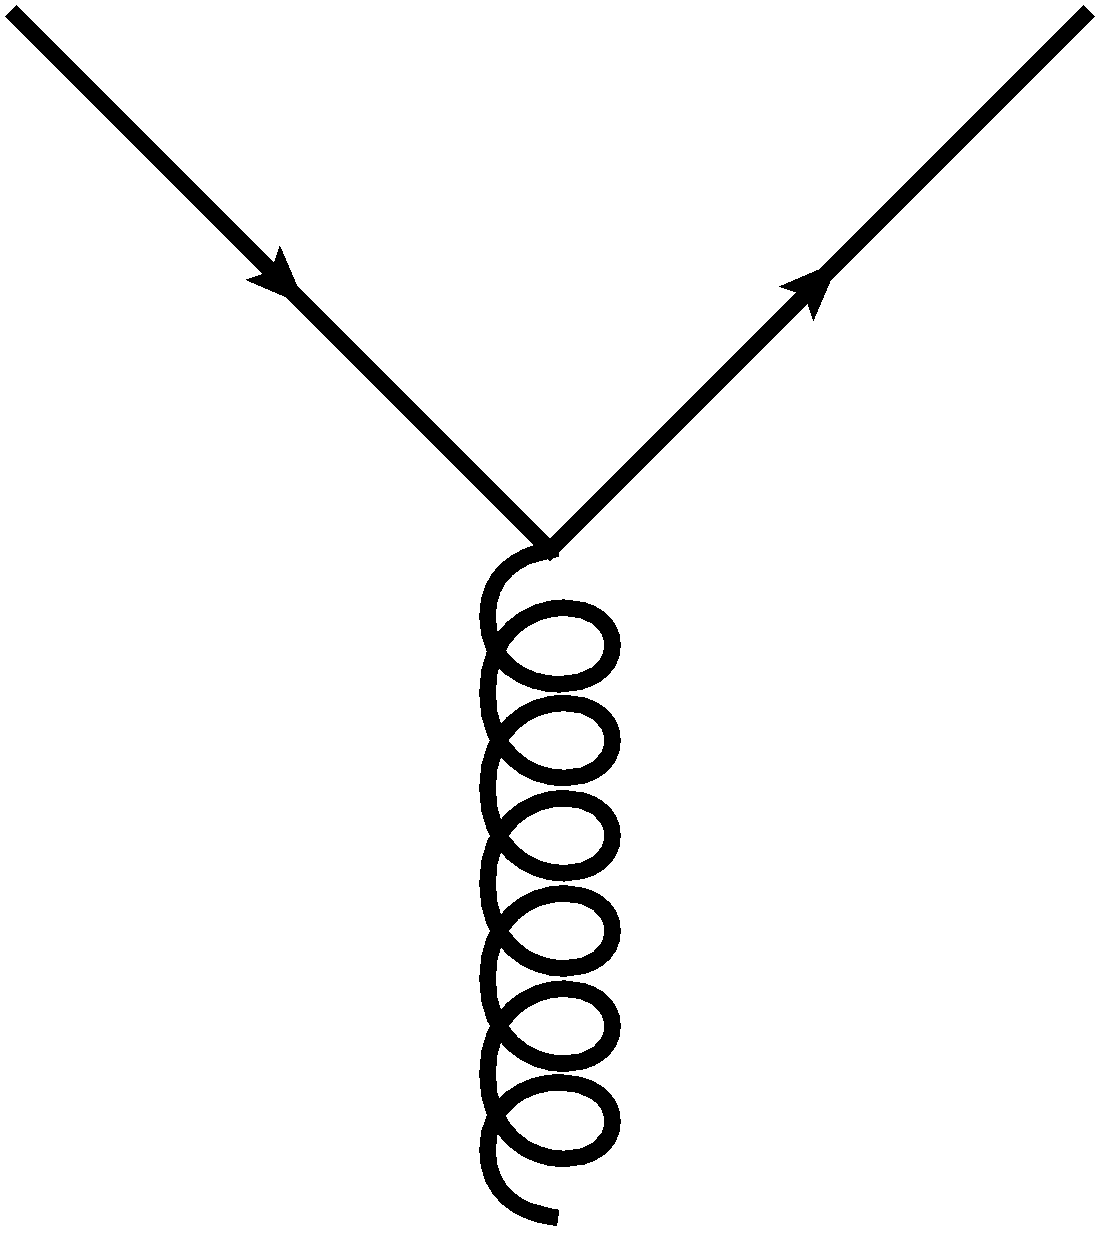
\includegraphics[width=0.3\textwidth]{figures/sm_model/fund_2.png}
% 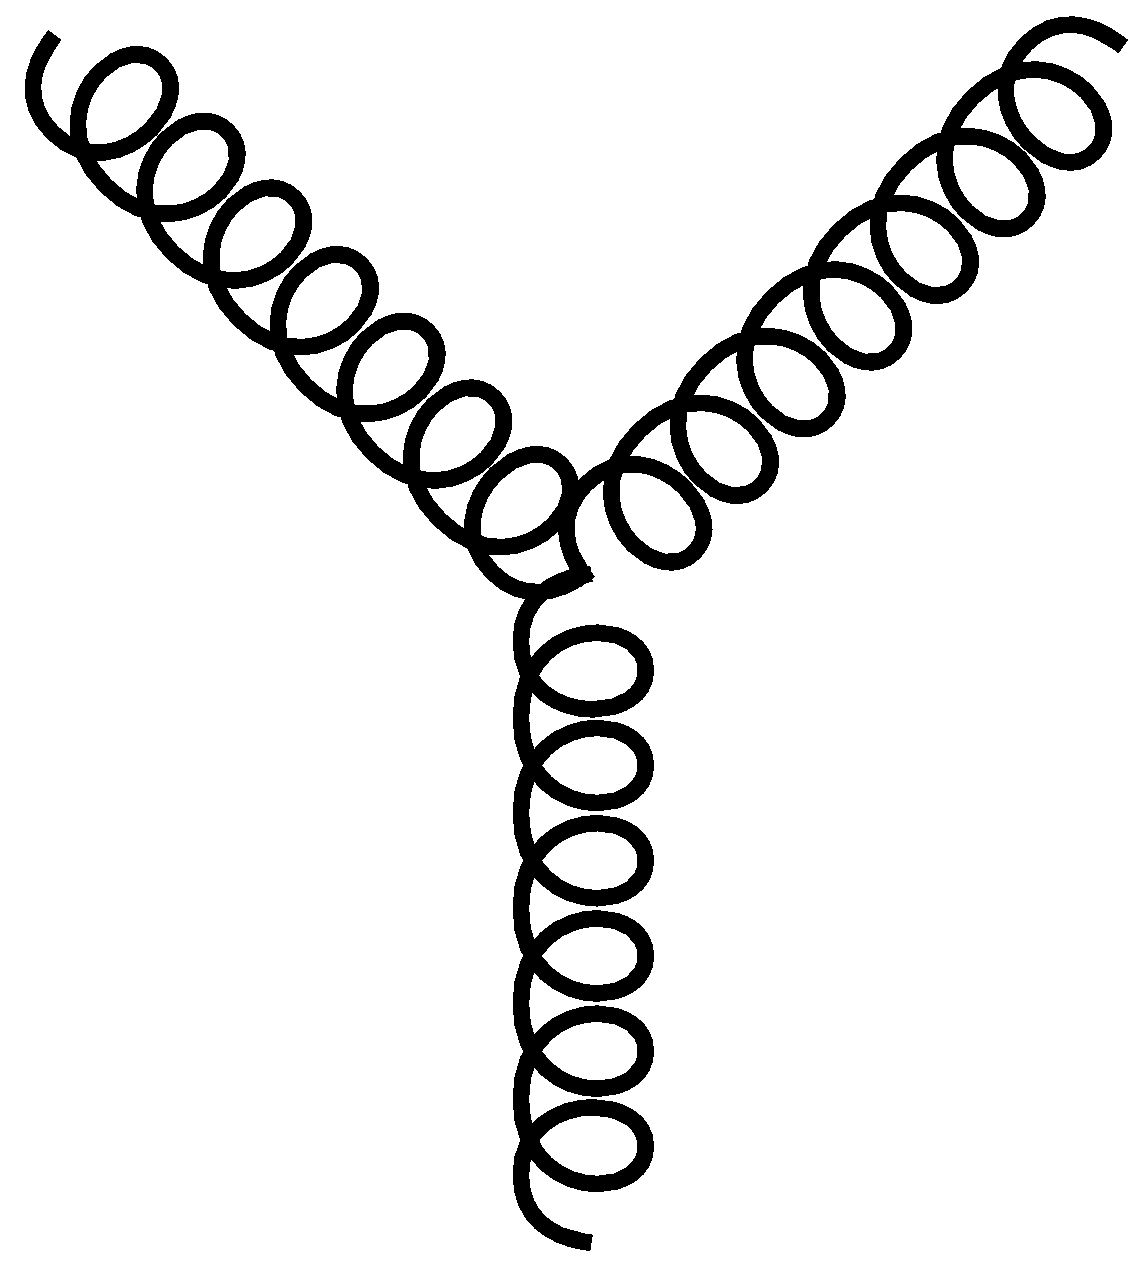
\includegraphics[width=0.3\textwidth]{figures/sm_model/fund_3.png}
% 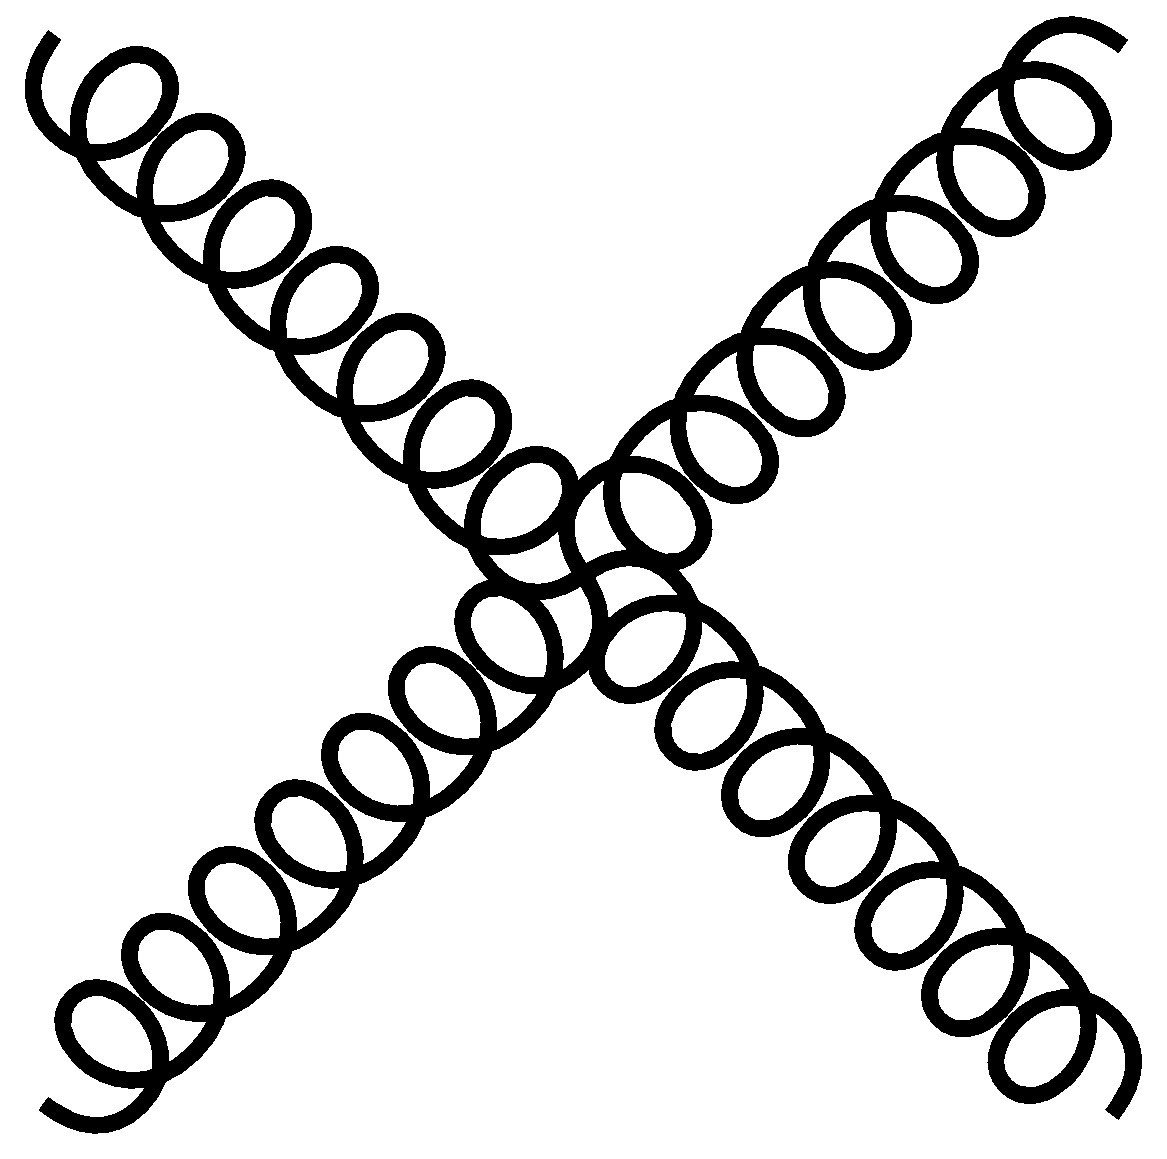
\includegraphics[width=0.3\textwidth]{figures/sm_model/fund_4.png}
% \caption[The fundamental couplings of the gluon.]{The fundamental couplings of the gluons:a) a quark interacting with a gluon and b,c) the gluon-gluon self-coupling. }
% \label{fig:fundamental:couplings}
% \end{figure}
%
%
% \subsection{The Running Coupling of the Strong Interaction}
%
% In analogy to quantum electrodynamics (QED) with the fine-structure constant
% $\alpha$, a coupling constant \as has been introduced for QCD.  The strong
% coupling constant describes the strength of the interaction between the gluon
% and the colour charge $g_s = \sqrt{4\pi \as}$. Just as in QED, the coupling
% constant is not energy-independent, but changes with the squared momentum
% transfer \q. The energy dependence is due to particles originating from vacuum
% fluctuations, which interact with the electrical charge or colour-charge. These
% interactions should lead to an increase of the strong coupling constant at
% higher \q. But in QCD the gluons couple to themselves, leading to a dominating
% anti-screening effect. Therefore, effectively \as decreases at small distances
% (i.e. high momentum transfers). 
%
% In processes with high momentum transfer, the coupling gets very small and the
% quarks can be regarded as free. This is also called \emph{asymptotic freedom}.
% However, if the momentum transfer is very small, the coupling can become very
% strong and perturbative techniques are not applicable anymore. Therefore all
% colour charges are bound together into colourless objects, and a separation of
% two coloured particles is not possible, but leads to the energetically more
% favourable creation of new colourless hadrons. This phenomenon is named
% \emph{confinement}.
%
% \subsubsection{Energy Dependence of \as}
%
% Physical observables can be written in a perturbative approach as an expansion
% in the strong coupling \as. Since it is possible that additional emissions and
% ultraviolet divergences arise, these have to be removed in a process called
% renormalisation. This introduces an additional energy scale $\mu$, and \as and
% physical observables get dependent on $\mu$. The fact that physical observables
% X do not depend on these scale is given mathematically by the renormalisation
% group equation (RGE):
%
% \begin{equation}
% \mu^2 \frac{d}{d \mu^2} X(\frac{q^2}{\mu^2},\as(\mu^2)) \stackrel{!}{=} 0 =
% \left( \mu^2 \frac{\partial}{\partial \mu^2} + \mu^2 \frac{\partial
% \as(\mu^2)}{\partial \mu^2} \frac{\partial}{\partial \as(\mu^2)} \right) X
% (\frac{q^2}{\mu^2},\as(\mu^2)
% \end{equation}
%
% The behaviour of the strong coupling constant can be explained by the
% introduction of a $\beta$-function
%
%
% \begin{equation}
% \frac{\partial \ln \as(\mu^2)}{\partial \ln \mu^2} = \frac{\beta(\as(\mu^2))}{\as(\mu^2)}
% \end{equation}
%
% A perturbative ansatz for the solution of the $\beta$ function is 
%
% \begin{equation}
% \beta(\as(q^2)) = - \frac{\beta_0}{4\pi} \as^2(q^2) -\frac{\beta_1}{8 \pi^2} \as^3(q^2) + \mathcal{O}(\as^4)
% \end{equation}
%
% The coefficients $\beta_i$ can be calculated within a given renormalisation
% scheme like the $\overline{MS}$~\cite{PhysRevD.18.3998} scheme. With a one-loop
% QCD calculation, and a given number of quark flavours $n_f$, $\beta_0$ can be
% expressed as
%
% \begin{equation}
% \beta_0 = \frac{33-2 n_f}{12\pi}
% \end{equation}
%
% \begin{equation}
% \beta_1 =\frac{153-19 n_f}{24 \pi^2}
% \end{equation}
%
% Solving the RGE equation for the one-loop solution of the $\beta$ function leads to
%
% \begin{equation}
% \as(q^2) = \frac{\as(\mu^2)}{1 + \as(\mu^2)\frac{\beta_0}{4 \pi} \ln(\frac{q^2}{\mu^2})}.
% \end{equation}
%
% To compare the strong coupling constant between different experiments, it is
% common usage to evaluate \as at $\mu^2= (M_Z)^2$. The results, which are
% available at next-to-next-to-leading-order (NNLO) precision, are combined into a
% world average value of \as. The Particle Data Group reports \as currently as
%
%
% \begin{equation}
% \as(M_Z^2) = 0.1184 \pm 0.0007.
% \end{equation}
%
%
% \begin{figure}[htb]
%     \centering
%   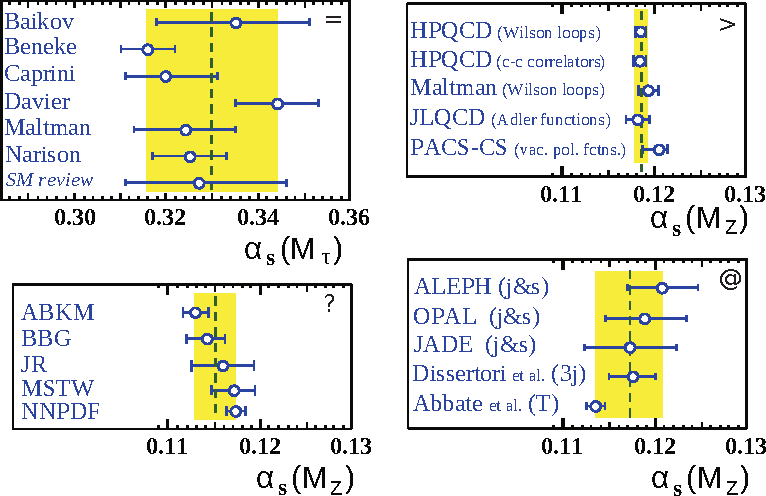
\includegraphics[width=1.0\textwidth]{figures/sm_model/alpha_s_measurements.pdf}
%      \caption[Determination of \asmz]{Summary of determinations of \as using
%          hadronic $\tau$-decays (a), from lattice calculations (b), from DIS
%          measurements (c) and from event shapes and jet production in $e^+e^-$
%          annihilation (d)~\cite{Beringer:1900zz}.}
% \end{figure}
%
% \begin{figure}[ht]
%     \centering
%   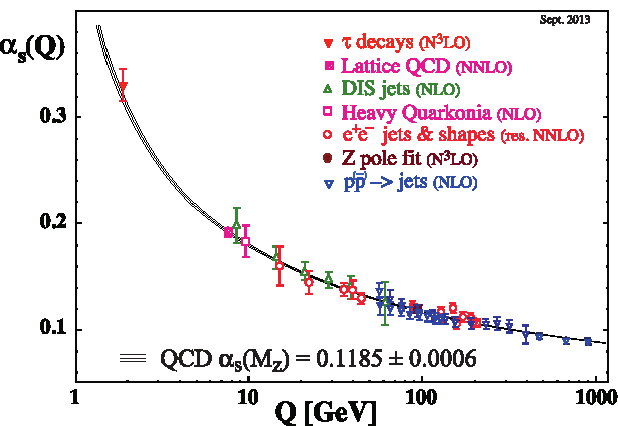
\includegraphics[width=1.0\textwidth]{figures/sm_model/as_running.pdf}
%      \caption[Running of \as]{Summary of measurements at different energies show
%          agreement with the predicted running behaviour of \as. The evolution to
%          the Z boson mass scale yields the current world average value $\asmz =
%          0.1184\pm 0.0007$~\cite{Beringer:1900zz}.}
% \end{figure}
%
% \subsection{Hadrons}
%
% The confinement ensures the colour neutral state of observable objects. Since
% separating quarks from each other needs more energy than the creation of another
% quark-antiquark pair, the quarks combine into colourless bound states. These are
% called hadrons and can be classified according to their constituents.
%
% \begin{description}
% \item[Mesons] consist of one quark and one anti-quark. They have spin-0 or spin-1 and are therefore bosons.
% \item[Baryons] consist of three quarks or anti-quarks. They have spin-$\frac{1}{2}$ and are fermions.
% \end{description}
%
% All hadrons except for the proton are unstable. The decay of a proton is
% studied, but has not yet been observed experimentally. The decay of such hadrons
% occur via the strong, weak or electro-magnetic interaction. 
%
% The properties of the proton have been studied very carefully at particle
% colliders. The ideal way to probe the substructure of the proton is looking at
% deep inelastic scattering (DIS) of electrons or positrons through the exchange
% of a virtual photon. Above an energy of around \SI{1}{\giga \electronvolt}, the
% inner substructure of the proton is revealed and it was found that the proton
% consists of point-like particles, the so-called partons. The behaviour of the
% substructure of the proton can be described very well in the parton-model and
% even better in the QCD improved parton model.  \vspace{\baselineskip}
%
% In DIS processes, the deviation from elastic scattering is described using the
% Bjorken scaling variable $x$. $P$ is the four-momentum of the proton with the
% mass $M$. The quantities $k$ and $k'$ are the four-momentum of the incoming and
% outgoing lepton. The exchanged particle transfers the four momentum $q$ =
% $k-k'$. The Lorentz invariant energy transfer is $\nu = \frac{Pq}{M_h}$. 
%
% \begin{equation}
% x = \frac{Q^2}{2 M_h \nu} = \frac{Q^2}{2 P q}
% \end{equation}
%
% In early publications at an energy of around \SI{3}{\giga \electronvolt}, it was
% shown, that the scaling behaviour $x$ is independent of $Q^2$. If the scattering
% occurs between spin-$\frac{1}{2}$ particles, the measured structure functions
% $F_1$ and $F_2$ can be related through the Callan-Gross relation, which is only
% valid for fermionic objects.
%
% \begin{equation}
% 2x F_1(x) = F_2 (x)
% \end{equation} 
%
% The DIS experiments confirmed that quarks are fermions. At higher momentum
% transfers, the parton masses can be neglected and the Bjorken scaling variable
% $x$ can be interpreted as the momentum fraction of the proton carried by one of
% the constituents. The momentum fraction carried by the parton i can be written
% as probability function $f_i(x_i)$. It was found that only half of the momentum
% of the proton is carried by the quarks. The question about the missing momentum
% has been solved by the QCD improved parton model which includes also the gluons
% as additional momentum-carrying partons.
%
% \subsection{QCD Improved Parton Model}
%
% In contrary to the naive assumptions of independent parton constituents in the
% quark parton model, the QCD improved parton model includes interactions between
% partons through the exchange of gluons. If the momentum transfer \q is large
% enough for \as to be treated in a perturbative approach calculations can be
% performed.
%
% However the cross sections cannot be completely calculated in a perturbative
% approach. An important property of the theory is the ability to factorise the
% cross section into a hard scattering matrix element and the parton distribution
% functions. With short-range hard matrix element $\hat \sigma$, which is
% calculable in perturbative QCD, and the long-range parton distribution functions
% $f_a$ and $f_b$, the full cross section can be written as:
%
% \begin{equation}
% \sigma(x,Q^2) = \sum_f \int_{x_1,x_2}^1 dx_1 dx_2 f_a(x_1,\mu_F^2) f_b(x_2,\mu_F^2) \times \hat \sigma_{ab \rightarrow X} (\q, \mu_F, \mu_R) 
% \end{equation}
%
%
% However, through this separation, the PDFs is no longer scale independent, as
% gluons can be radiated. Dorkshitzer, Gribov, Lipatov, Altarelli and Parisi
% introduced the DGLAP evolution equations, which describe the impact on the PDFs
% due to changes in \q~\cite{Dokshitzer:1977sg,Gribov:1972ri,Altarelli:1977zs}.
% The PDFs themselves cannot be calculated in perturbative calculations, but have
% to be derived from experimental measurements.
% \vspace{\baselineskip}
%
% To compare the measurements at different scales, a PDF of a gluon or quark is
% defined at a low scale and then evolved to the experiment specific scale using
% the DGLAP evolution equations:
%
% \begin{equation}
% \frac{\partial q(x,\mu^2)}{\partial \log \mu^2} = \frac{\as}{2 \pi} \int_x^1 \frac{dz}{z} \left( P_{q \rightarrow q g}(z,\as)q \left(\frac{x}{z},\mu^2 \right) + P_{g  \rightarrow q q}(z,\as)g \left(\frac{x}{z},\mu^2 \right) \right)
% \end{equation}
% \begin{equation}
% \frac{\partial g(x,\mu^2)}{\partial \log \mu^2} = \frac{\as}{2 \pi} \int_x^1 \frac{dz}{z} \left( P_{q \rightarrow qg}(z,\as)q \left(\frac{x}{z},\mu^2 \right) + P_{q \rightarrow gg}(z,\as)g \left(\frac{x}{z},\mu^2 \right) \right)
% \end{equation}
%
% $z$ is the momentum fraction of the parton after radiation of the gluon, while
% the splitting functions $P_{a \rightarrow bc}(z,\as(\mu^2))$ describe the
% probability of radiation. The splitting function can be evolved in orders of \as
% as
%
% \begin{equation}
% P_{ab}(x;\as(\mu^2)) = P_{ab}^0(x) + \frac{\as}{2\pi}P_{ab}^1(x) + O(\as^2)
% \end{equation}
%
%
% The effect of the evolution can be seen from the comparison of a PDF at a low
% scale and a high scale. Figure \ref{fig:pdffit} shows the fitted PDF at a scale
% of $Q^2 = \SI{10}{GeV^2}$ and $Q^2 = \SI{200}{GeV^2}$. The gluon splitting leads
% to a strong rise of the gluon PDF and also to a small increase of the quark PDFs
% in the low-$x$ region when the PDF is evolved to higher scales.
%
% \begin{figure}[htb]
% \centering
% 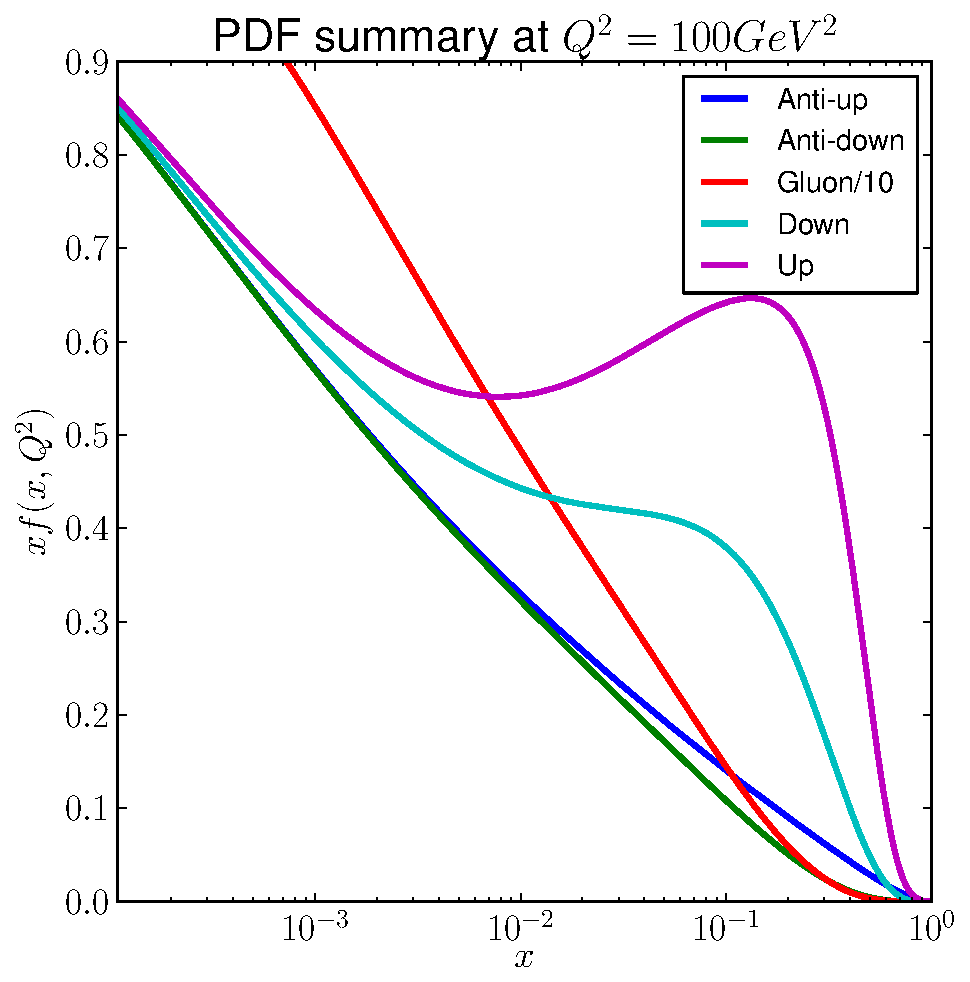
\includegraphics[width=0.48\textwidth]{figures/sm_model/summary_10.pdf}
% 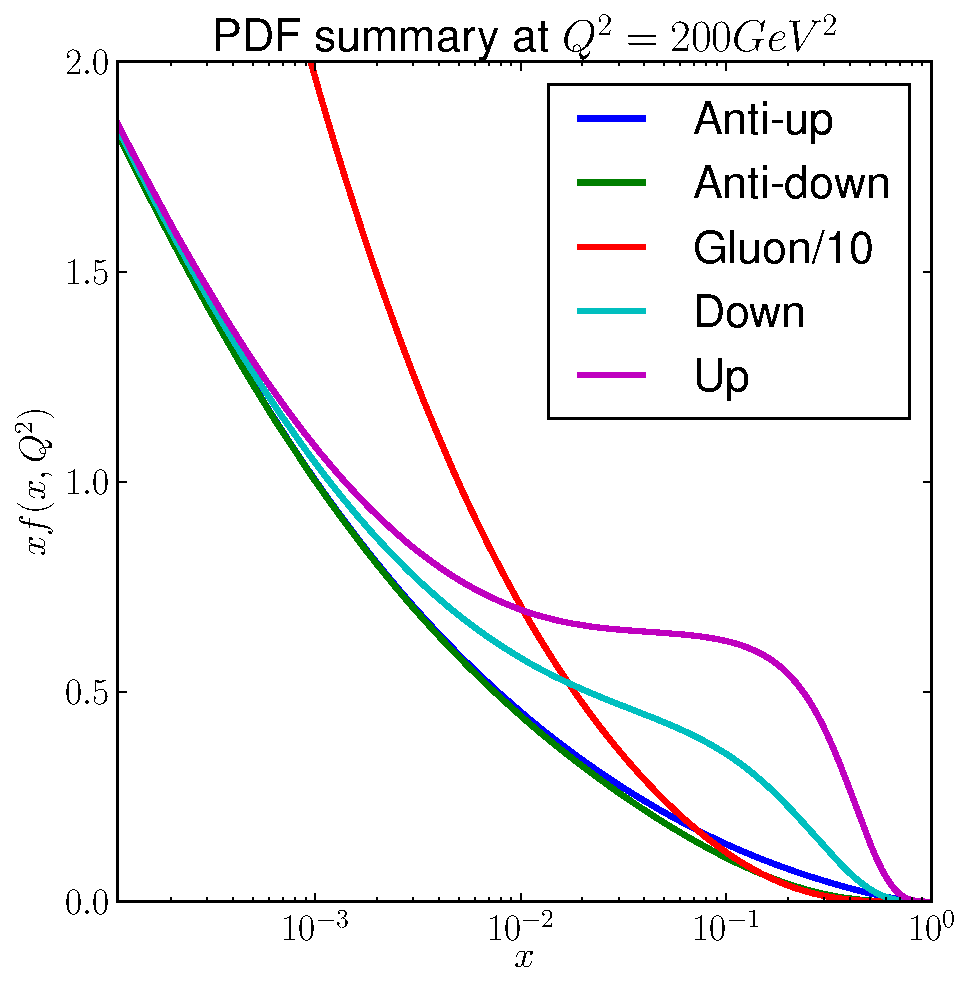
\includegraphics[width=0.48\textwidth]{figures/sm_model/summary_200.pdf}
% \caption[Parton distribution functions.]{Parton distribution functions at
% different scales. Presented is an own fit produced with the HERAFitter framework
% using HERA DIS and CMS Inclusive jet data.}
% \label{fig:pdffit}
% \end{figure}
%
% As each experiment can only cover a specific region of the phase space, it is
% important to combine data from different experiments to measure the PDF with the
% highest possible precision. Currently the global PDF studies combine data of the
% HERA and the Tevatron colliders as well as data from fixed-targets experiments.
% The covered range in $x$ and \q of each experiment is shown in Figure
% \ref{kinematic_plane}.
%
%
% \begin{figure}[htb]
%     \centering
%   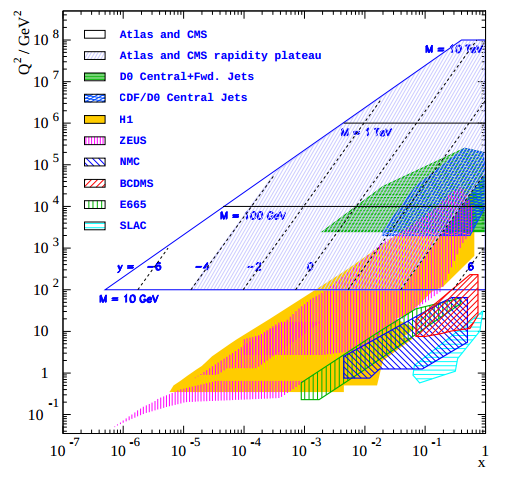
\includegraphics[width=1.0\textwidth]{figures/sm_model/kinematic_plane.png}
%      \caption[Kinematic plane]{Accessible phase space region for different
%          experiments. The HERA data covers a wide range in $x$ and \q and
%          therefore is included in all fits as base data set. LHC data allows to
%          probe the PDFs at high scales and covers the remaining $x$ region close
%          to 1.0~\cite{Glazov:2007zz}.}
%      \label{kinematic_plane}
% \end{figure}
%
% Many different groups extract these PDF sets from published data using different
% approaches. The groups MSTW~\cite{Martin:2009iq}, CTEQ~\cite{Lai:2010vv},
% NNPDF~\cite{Ball:2010de} and ABM~\cite{Alekhin:2012du} use data sets from all
% available experiments while the HERAPDF group~\cite{Aaron:2009aa} uses only data
% from the HERA collider. Due to the combination of datasets from many different
% sources, this poses also an important cross check of the compatibility between
% these data sets. More details on each PDF can be found in the cited publication
% by the respective PDF group.
%
% \section{Cross Sections}
%
% In order to verify the predictions made by pQCD, one needs an observable to
% compare the measurement to the calculation. The cross section $\sigma$ is such
% an observable. It is defined as the interaction rate per target particle $W$
% normalised to the particle flux $\Phi$:
%
% \begin{equation}
% \sigma = \frac{W}{\Phi}
% \end{equation}
%
% The comparison between the theoretically derived and the measured cross section
% gives some indications of the goodness of the used model, or also might contain
% hints on new physics. The commonly used unit of the cross section is a
% \emph{barn}, with $\SI{1}{\barn} = \SI{e-28}{\metre \squared}$. It is often
% useful to define the cross section differentially, e.g. in terms of transverse
% momentum \pt and the rapidity $y$ as it has been done for the inclusive jet
% cross section.
% \vspace{\baselineskip}
%
% The interaction rate W can be calculated with Fermi's Golden Rule, which uses
% the quantum-mechanical transition matrix elements $|M_{fi}|$ between initial and
% final state and the energy density $\rho_f$ of the final states.
%
%
% \begin{equation}
% W = \frac{2}{\pi} \mid M_{fi}^2 \mid \rho_f
% \end{equation}
%
% The properties of the collider are related to the number of produced events. 
%
% \begin{equation}
% \sigma = \frac{W}{L}
% \end{equation}
%
% Therefore, the instantaneous luminosity L is defined, which contains for the LHC
% quantities like the numbers of protons per bunch, the properties of the beam
% optics and the energy. 
% The actually used luminosity is measured experimentally by relating the nuclear
% elastic forward scattering amplitude with the total cross section. The absolute
% luminosity scale is determined using Van der Meer scans. This procedure scans
% the LHC beams through one another to measure the size of the beams at the
% collision point.
%
%
